\documentclass{article}
\usepackage{amsmath}
\usepackage{tikz}
\usetikzlibrary{bayesnet}
\DeclareMathOperator*{\argmax}{arg\,max}
\renewcommand\phi\varphi

\begin{document}


\textbf{Notation:}
\begin{table}[h]
\begin{tabular}{ll}
$N$                   & number of VSO triples (indexed by $i$)                      \\
$F$                   & number of frames (indexed by $f$)                       \\
$V^a$                 & vocabulary size of argument $a$\\
$f$                   & the sequence of frames (one for each triple)        \\
$f_i$                 & $1\leq f_i\leq F$ is the frame assigned to the $i$th triple      \\
$w$           & the sequence of VSO triples (this is our data)                               \\
$ w_i$            & $i$th triple                                            \\
$w_i^{a}$           & the word from argument $a$ ($a\in\{s,v,o\}$) in the $i$th triple \\
$\phi$          & sequence probability distributions characterizing frames    \\
$\phi_f$          & probability distributions for frame $f$                  \\
$\phi_f^{a}$        & probability distribution for syntactic role $a$ in frame $f$ \\
$C(w,f,a)$          & number of times that $w$ appears in position $a$ in triples assigned to frame $f$\\
\end{tabular}
\end{table}

The generative story for model 0 is

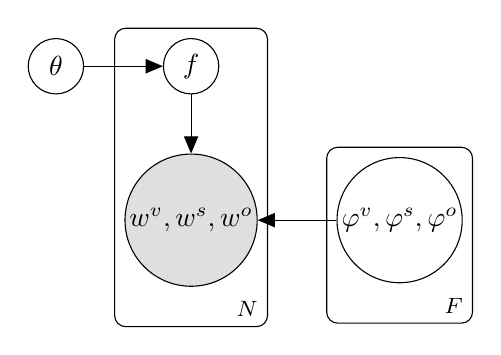
\begin{tikzpicture}
  % Nodes
  \node[obs] (datapoint) {$w^v,w^s,w^o$} ; %
  \node[latent, above=0.75cm of datapoint] (F) {$f$} ; %
  \node[latent, left=of F] (theta) {$\theta$}; %
  \node[latent, right=of datapoint] (phi) {$\varphi^v,\varphi^s,\varphi^o$}; %
  \edge {theta} {F} ; %
  \edge {F} {datapoint}
  \edge {phi} {datapoint} ; %
  \plate {tuples} {(F) (datapoint) } {$N$}; %
  \plate {} {(phi)} {$F$} ; %
\end{tikzpicture}


\[
P(f,w,\phi|\theta,\beta)
= P(f|\theta)P(w|\phi)P(\phi|\beta)
\]

\begin{align*}
P(f|\theta)      =& \prod_{i=1}^{N}P(f_i|\theta)\\
P(w|\phi,f)      =& \prod_{i=1}^N\prod_{a}^{\{v,s,o\}}P(w_i^a | \phi_{f_i}^a)\\
                 =& \prod_{f=1}^{F}\prod_{w=1}^{V}\prod_{a}^{\{s,v,o\}}P(w|\phi_f^a)^{C(w,f,a)}\\
P(\phi|\beta)    =& \Big(\frac{3}{B(\beta)}\Big)^K\prod_{f=1}^{F}\prod_{w=1}^{V}\prod_{a}^{\{s,v,o\}}P(w|\phi_f^a)
\end{align*}

So we have...

E-step:
\begin{align*}
\mu_i(f) =& P(f|w_i)\\
         =& \frac{P(w_i|f)P(f)}{P(w_i)}\\
         =& \frac{\prod_a^{\{v,s,o\}}P(w_i^a|\phi_f^a) P(f|\theta)}{\sum_{f'}^F\prod_a^{\{v,s,o\}}P(w_i^a|\phi_{f'}^a)}
\end{align*}

M-step:
\begin{align*}
E_\mu[\sum_{i=1}^N\log P(w_i,f_i|\theta,\phi)]
        =& \sum_{i=1}^N E_\mu[\log P(w_i,z_i|\theta,\phi)] \\
  \approx& \sum_{i=1}^N \sum_{f=1}^F\mu_i(f)\log P(w_i,f|\theta,\phi) 
                 \tag{estimates from E-step}\\
  \approx& \sum_{i=1}^N \sum_{f=1}^F\mu_i(f)\log P(f|\theta) \prod_a^{\{v,s,o\}}P(w_i^a|\phi_f^a)
                 \tag{estimates for $\phi$, $\theta$}  \\
        =& \sum_{i=1}^N \sum_{f=1}^F\mu_i(f)\log P(f|\theta) + \sum_{i=1}^N \sum_{f=1}^F\mu_i(f)\log \prod_a^{\{v,s,o\}}P(w_i^a|\phi_f^a)\\
        =& \sum_{i=1}^N \sum_{f=1}^F\mu_i(f)\log P(f|\theta) + \sum_{i=1}^N \sum_{f=1}^F \sum_a^{\{v,s,o\}} \mu_i(f)\log P(w_i^a|\phi_f^a)\\
\end{align*}

% TODO: show the lagrange derivations
\begin{align*}
\argmax_{\theta(f)}\sum_{i=1}^N \sum_{f=1}^F\mu_i(f)\log P(f|\theta)
    =& \frac{\sum_{i=1}^N \mu_i(f)}{\sum_{f'=1}^F\sum_{i=1}^N\mu_i(f')}
\end{align*}

\begin{align*}
\argmax_{\phi^a_f(w)} \sum_{i=1}^N \sum_{f=1}^F \sum_a^{\{v,s,o\}} \mu_i(f)\log P(w_i^a|\phi_f^a)
    =& \frac{\sum_{i=1}^N \mu_i(f) C(w,a)}{\sum_{w'=1}^{V^a}\sum_{i=1}^N \mu_i(f) C(w',a)}
\intertext{Where $C(w,a)$ is the number of times w appears as argument $a$.}
\end{align*}

\end{document}
